\section{Versuchsaufbau/-durchführung}
\begin{figure}
  \centering
  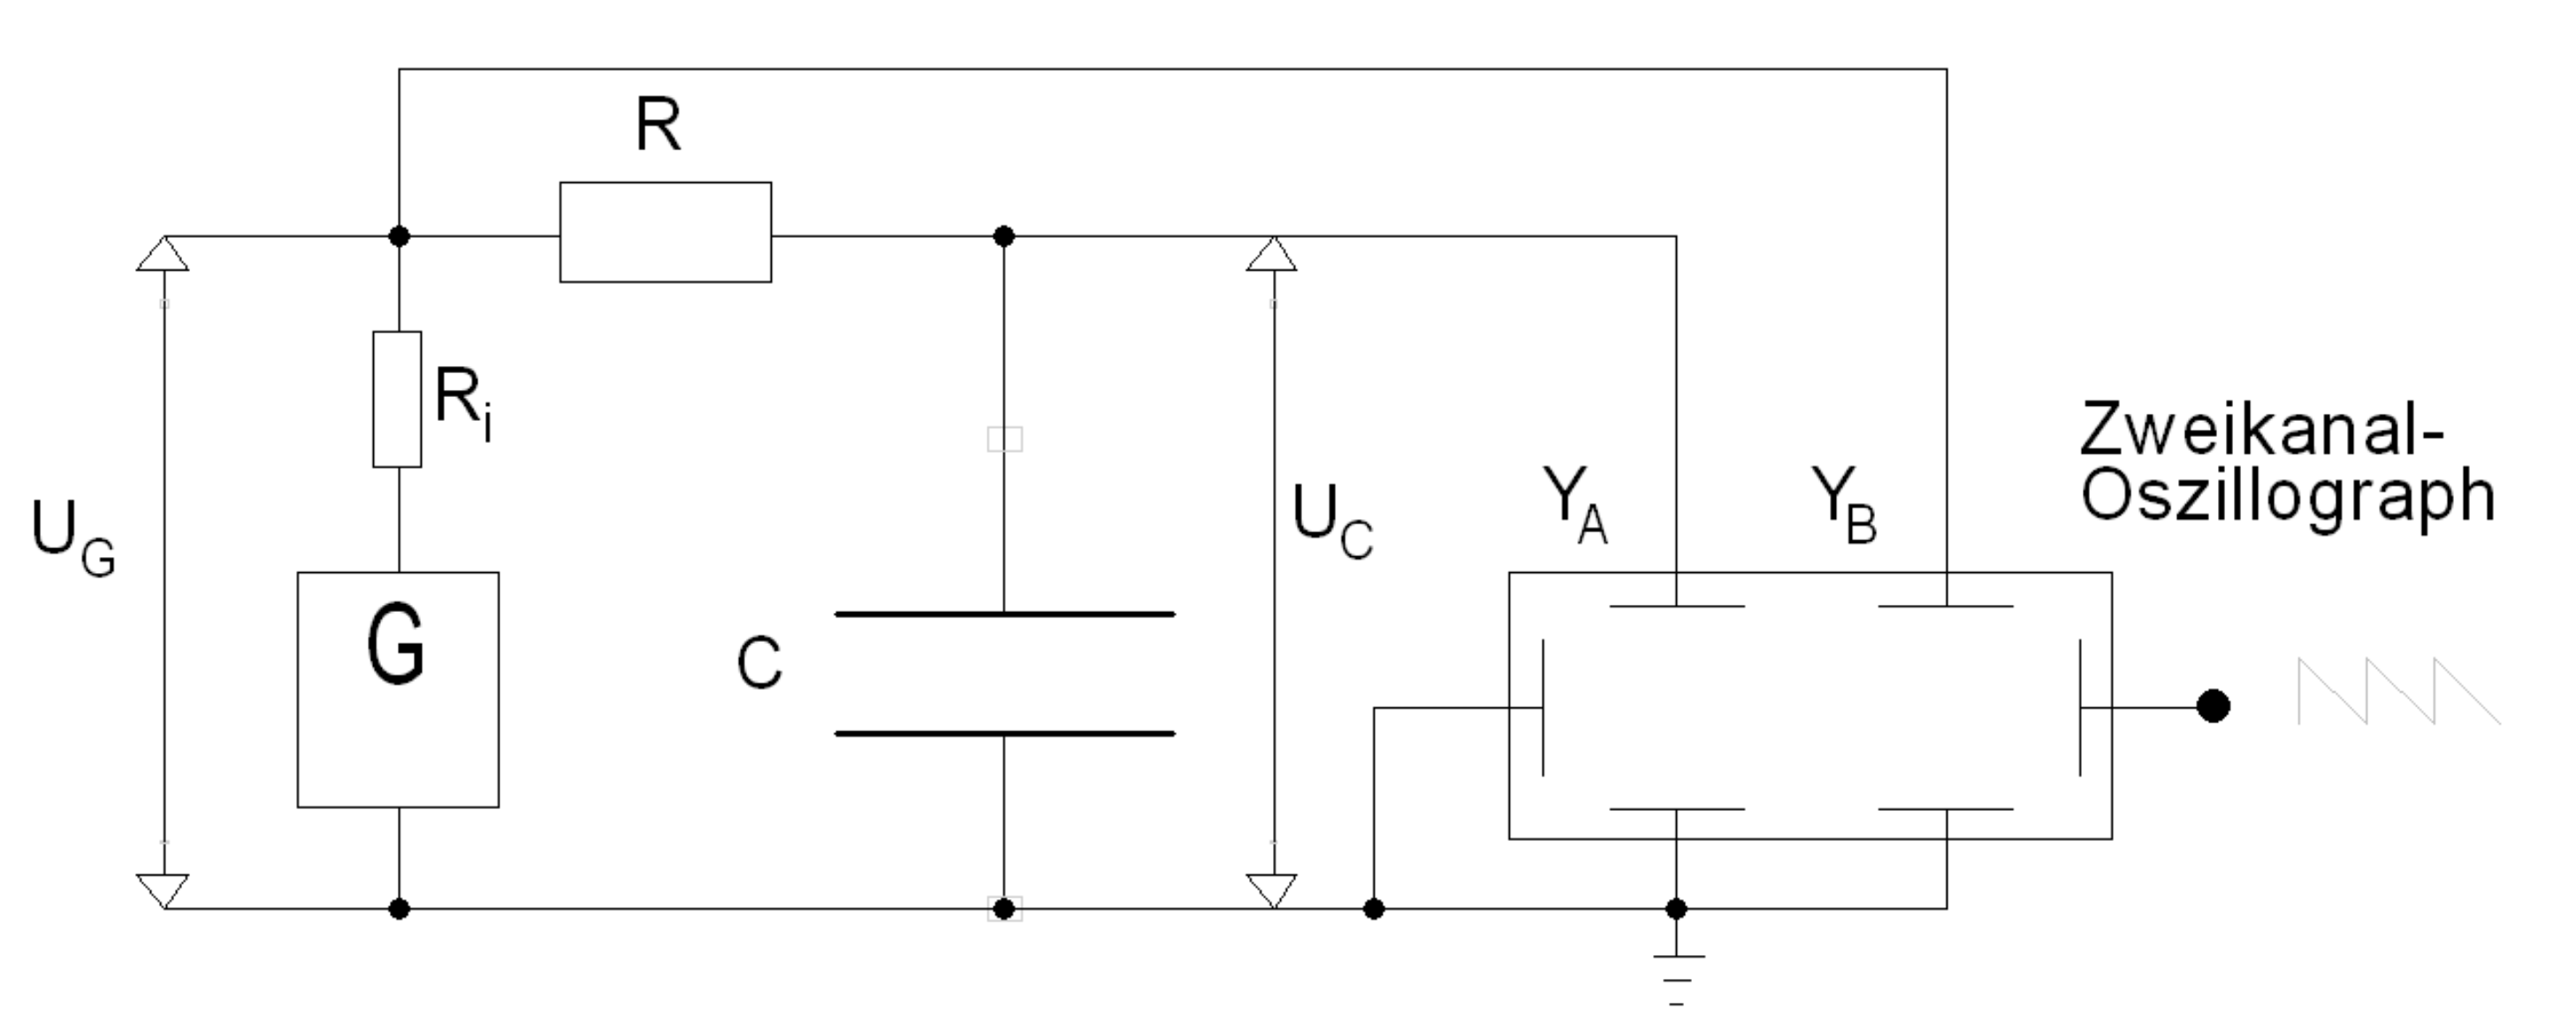
\includegraphics[width = \textwidth]{pics/aufbau.pdf}
  \caption{Verwendeteter Aufbau zur Untersuchung der Turbomolekularpumpe und Drehschieberpumpe.
Tank 1; Verbindungsstück 2; Nadelventil 3; Glühkathodenmessgerät 4;
Ventile 5, 6, 11; Schläuche 7, 12, 13; Turbomolekularpumpe 8; Steuereinheit für die Turbomolekularpumpe 14;
Pirani-Messgerät 10; Digitales Pirani-Messgerät (außer Betrieb) 9; Analoge Anzeigegeräte für Pirani und Glühkathodenmessgerät 15.}
  \label{fig: aufbau}
\end{figure}
Der verwendete Aufbau zur Bestimmung des realen Saugvermögens einer Turbomolekular und Drehschieberpumpe ist in
Abbildung~\ref{fig: aufbau} einzusehen. Hierbei ist der Schlauch 13 mit der Drehschieberpumpe verbunden, die seperat in
Abbildung~\ref{fig: aufbaudrehschieber} dargestellt ist.

Um den Aufbau auf Dichtigkeit zu überprüfen und um eventuelle Wasseranlagerungen an der Innenseite des Rezipienten zu entfernen,
wird zunächst mit der Drehschieberpumpe ein Vorvakuum erzeugt und anschließend die Turbomolekularpumpe in Betrieb genommen. Mit Hilfe
eines Heißluftföns wird der Tank erwärmt, was zur Desorption von Anlagerungen führen soll. Anschließend kann mit der Untersuchung der
Drehschieberpumpe begonnen werden.
\subsection{Untersuchung der Drehschieberpumpe}
Die Ventile 5 und 11 werden geschlossen, sodass die Turbomolekularpumpe vom Aufbau isoliert wird. Durch Öffnen des Nadelventils 3
wird in dem evakuierten Rezipienten ein Normaldruck erzeugt, der als Startwert $p_0$ für die Aufzeichnung des zeitlichen Druckverlaufs
$p(t)$ verwendet wird. Zur Zeit $t = 0$ wird in mehreren Durchlaüfen das Nadelventil geschlossen
und mit Hilfe eines Smartphones die Zeit $t\ua{i}$ zu festen Druckwerten $p\ua{i}$ aufgenommen. Zur Druckmessung wird das Piranimessgerät
verwendet.

Wie in der Theorie beschrieben kann das Saugvermögen $S$ ebenfalls durch eine Leckratenmessung bestimmt werden. Hierzu wird zunächst mit
dem Nadelventil ein Gleichgewichtsdruck $p\ua{G}$ eingestellt. Zur Zeit $t = 0$ wird das Ventil 16 geschlossen und der zeitliche
Druckanstieg aufgezeichnet. Das Verfahren wird für mehrere Gleichgewichtsdrücke durchgeführt.

\begin{figure}
  \centering
  \includegraphics[width = 0.6\textwidth]{pics/drehschieberpumpe.pdf}
  \caption{Unterer Teil des Versuchsaufbaus. Drehschieberpumpe 17 und Ventil 16.}
  \label{fig: aufbaudrehschieber}
\end{figure}
\FloatBarrier
\subsection{Untersuchung der Turbomolekularpumpe}
Die Ventile 11 und 5 werden geöffnet, Ventil 6 geschlossen. Die Drehschieberpumpe dient in diesem Teil des Versuchs als
Vorpumpe, mit der ein Druck im Bereich $p\propto \SI{0.1}{\milli\bar}$ erzeugt wird. Mit der Steuereinheit 14 wird die Drehzahl der
Turbomolekularpumpe auf $\SI{1350}{\hertz}$ erhöht. Als Druckmessgerät wird das Glühkathodenvakuummeter verwendet. Um den Enddruck $p\ua{E}$
zu bestimmen, wird die Turbomolekularpumpe für einige Zeit $\propto \SI{20}{\minute}$ betrieben. Anschließend kann analog zu den Untersuchungen der
Drehschieberpumpe der zeitliche Verlauf des Drucks $p(t)$ sowie die Leckrate aufgenommen werden.

\subsection{Volumenmessung}
Beim Demontieren des Aufbaus werden die Maße der Einzelteile vermessen, um in der Auswertung das Gesamtvolumen des Rezipienten zu bestimmen. Da der Tank
1 nicht aufgeschraubt werden soll, kann hier nur eine Messung des Außenvolumens erfolgen. Für die anderen Teile werden möglichst genau
die relevanten Größen zur Berechnung des Innenvolumens aufgenommen. Hierzu wird ein Messschieber werwendet.
